Cliquez sur le centre de vacances pour lequel vous souhaitez demander des subsides. 
Pour envoyer une demande de subsides, il est nécessaire de compléter entièrement les trois onglets suivants: \ovalbox{Encadrement}, \ovalbox{Présences}, \ovalbox{Enfants}.


\begin{figure}[h!]
    \centering
    
\includegraphics[width=16cm]{Images/cdv/cdv-onglets-ds.png}
    \caption{Pour envoyer une demande de subside, il faut avoir complété préalablement les onglets encadrements, présences et enfants.}
    \label{fig:cdv_onglets}
\end{figure}



\subsection{DS (1/4) - L'onglet Encadrement}\label{encadrementcdv}

\begin{figure}[h!]
    \centering
    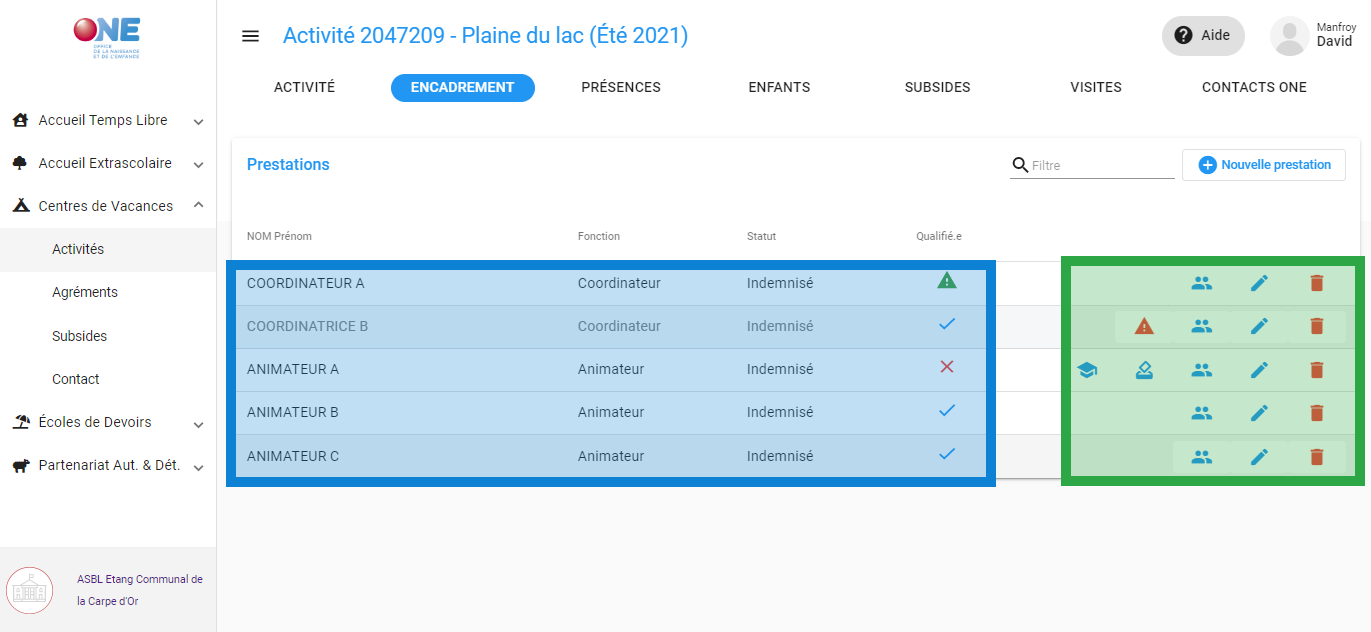
\includegraphics[width=15cm]{Images/cdv/cdv-ds-encadrement2.png}
    \caption{Onglet encadrement: liste du personnel qui preste pour l'activité}
    \label{fig:cdv_encadrement}
\end{figure}

Cet onglet reprend le personnel d'encadrement qui preste pour  votre activité centre de vacances (fig. \ref{fig:cdv_encadrement}. Vous renseignerez les coordinateurs et les animateurs qui ont animé les enfants (en \textcolor{bleu}{bleu}). Pour chacun d'eux, vous pourrez renseigner leur fonction (coordination ou animation), leur statut (indemnisé ou volontaire) et les qualifications pour leur fonction (qualifié ou non qualifié).

\subsubsection{Prestation, qualification ou suppression}
Quelques boutons d'action sont disponibles en \textcolor{vert}{vert} dans la fig. \ref{fig:cdv_encadrement}:

\begin{itemize}
    \item Si la personne est non-qualifiée, ses \textbf{qualifications} peuvent être renseignées en cliquant sur 
\includegraphics[width=0.3cm]{Images/icon/button_dmd_qualif.png}.
    \item Les informations de \textbf{prestation} (fonction et statut) sont modifiables en cliquant sur 
\includegraphics[width=0.3cm]{Images/icon/button_modif.png}.
    \item Vous avez également la possibilité de \textbf{supprimer la prestation} en cliquant sur 
\includegraphics[width=0.3cm]{Images/icon/icon-del.png}. Celle-ci n'apparaîtra alors plus dans le personnel de votre activité et ses données de présences seront supprimées (onglet présence).
\end{itemize} 


\subsubsection{Ajouter un membre du personnel}
Cliquez sur \ovalbox{Ajouter une prestation} en haut à droite. Dans l'encadré \fbox{\textbf{Nouvelle prestation}} (fig. \ref{fig:cdv_new_prestation}), vous serez invité à ajouter l'encadrant, à indiquer le contexte de sa prestation (contrat de travail, étudiant, stage ou convention de volontariat par exemple), sa fonction et son statut. 

\begin{figure}
    \centering
    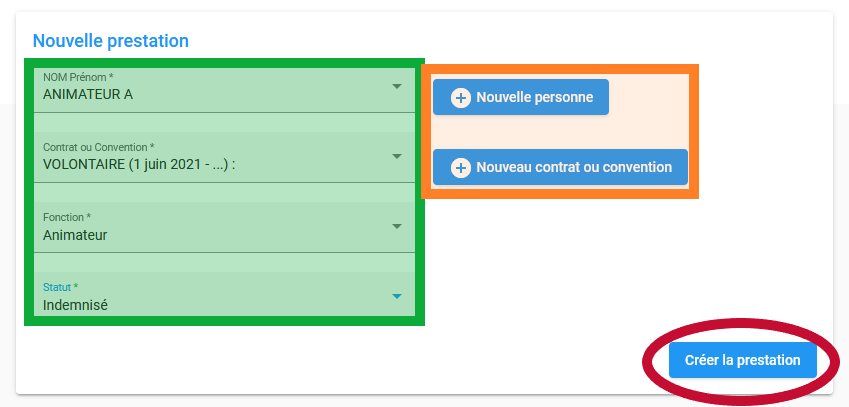
\includegraphics[width=10cm]{Images/cdv/new_prestation.png}
    \caption{Cadre Nouvelle prestation}
    \label{fig:cdv_new_prestation}
\end{figure}


\begin{enumerate}
    \item En cliquant sur "\textbf{prénom nom}*", vous aurez accès à la liste des personnes qui ont déjà travaillé pour votre pouvoir organisateur dans un centre de vacances;  sélectionnez ensuite la personne dans la liste. Si par contre, la personne ne figure pas dans la liste, cliquez sur \ovalbox{Ajouter une personne}. Vous serez alors dirigé vers "Mon Équipe" pour créer la personne (NISS + Prénom + Nom) et son lien contractuel avec votre Pouvoir organisateur. 
    \begin{conseil}
     Pour vous aider, suivez le point \ref{team_add_person} "Ajouter une personne dans Mon Équipe".
    \end{conseil}
    
    \item En cliquant sur "\textbf{Contrat et convention}", la liste vous donnera l'ensemble des liens (contractuels ou conventionnels) que la personne entretient avec votre pouvoir organisateur. La liste ne vous affichera que les contrats/conventions qui sont actifs: les dates du contrat doivent croiser celles de l'activité. 
    \begin{conseil}
     Pour vous aider, suivez le point \ref{team_add_contract} "Ajouter un contrat/un lien".
    \end{conseil}    
    
    
    \item Ajoutez la \textbf{fonction}: animateur ou coordinateur. 
        \begin{attention}
         Si la personne anime un jour et coordonne le centre un autre jour, il sera nécessaire de l'encoder deux fois. La personne ne pourra pas détenir les deux fonctions pour un même jour (il anime ou il coordonne, mais pas les deux au niveau du calcul de la subvention), mais il peut animer un jour et coordonner un autre jour.
        \end{attention}
    
    
    \item Indiquez le \textbf{statut de la personne}: indemnité ou volontaire. Ces champs seront pré-remplis en fonction du point 2 (contrat et convention), mais pourront être modifiés. 
    \item Cliquez enfin sur \ovalbox{Créer la prestation}. La personne sera alors ajoutée à la liste des encadrants de votre activité.
\end{enumerate}

\vspace*{4mm}
\begin{tcolorbox}[title=La personne ou le contrat/convention de celle-ci n'apparaît pas dans la liste]
La liste reprend les informations encodées dans "Mon Équipe":
\begin{itemize}
    \item Pour les personnes: elles doivent avoir été ajoutées dans Mon Équipe. Elles doivent en outre avoir un contrat en lien avec le secteur Centre de vacances encodées dans mon Équipe.
    \item Pour les contrats/conventions: la liste ne reprendra que les contrats/conventions dont les dates se chevauchent avec les dates de fonctionnement de votre activité centre de vacances.
\end{itemize}

Si les éléments que vous recherchez ne sont pas présents, cliquez sur \ovalbox{Créer une personne} ou \ovalbox{Créer un nouveau contrat/convention}. Suivez le point \ref{team_add_person} "Ajouter une personne dans Mon Équipe" et le point \ref{team_add_contract} "Ajouter un contrat/un lien" (chapitre \ref{chap:team} de ce Guide). 

\textbf{Remarque}: il sera peut être nécessaire non pas de créer un contrat (au risque d'avoir plusieurs même contrat encodée), mais d'adapter un contrat déjà existant dans Mon Équipe. Pour cela, développez Accueil Temps Libre, cliquez sur Mon Équipe. Rendez-vous ensuite dans la fiche de la personne pour modifier son ou ses contrats.  
\end{tcolorbox}


\subsubsection{Consulter les qualifications de la personne}
Dans l'encadré \textcolor{vert}{vert} de la fig. \ref{fig:cdv_encadrement}, vous pouvez voir les qualifications de la personne connues par l'ONE:

\begin{itemize}
    \item [$\bullet$]\textbf{\textcolor{bleu}{V}}: la personne est qualifiée pour exercer sa fonction d'animation ou de coordination. 
    \item [$\bullet$]\textbf{\textcolor{rouge}{X}}: la personne n'est pas qualifiée\footnote{Vous avez certainement déjà renseigné les informations de qualifications (copie de brevet, assimilation, etc.) pour certains animateurs ou coordinateurs les années précédentes. Malheureusement pour des raisons techniques, nous n'avons pas pu charger ces informations dans la nouvelle base de données. Le Service Centres de vacances possède les informations, mais il sera nécessaire de les recommuniquer (via une demande de qualification) afin que nos agents puissent faire les vérifications nécessaires dans nos anciens fichiers. Une fois les vérifications faites, la personne sera à nouveau considérée comme qualifiée dans votre Portail Pro.}  pour exercer sa fonction d'animation ou de coordination. 
    \item [$\bullet$]
\includegraphics[width=0.3cm]{Images/icon/icon_sablier.png}: une demande de qualification est en cours d'analyse auprès de l'ONE. 
    \item [$\bullet$]
\includegraphics[width=0.4cm]{Images/icon/icon_attention.png}: la personne a obtenu sa qualification durant l'année en cours. En fonction de la date d'octroi de la qualification, le calcul de subventionnement peut être impacté. En effet, la personne est considérée comme non qualifiée avant cette date. 
\end{itemize}
\vspace*{3mm}

\begin{tcolorbox}[title=Les quatre possibilités de qualification CDV]
Pour le secteur Centres de vacances, la personne peut: 

\begin{enumerate}
    \item Être en possession d'un \textbf{brevet centres de vacances} délivré par un organisme de formation agréé;
    \item Rentrer dans les conditions pour être \textbf{assimilé à un animateur/coordinateur breveté} 
    \item Avoir un \textbf{numéro d'assimilation} déjà obtenu; 
    \item Être en possession d'une \textbf{équivalence au brevet} \textit{(le BAFA par exemple)}.
\end{enumerate}
Pour faire reconnaître cette qualification, il faut envoyer une demande de qualification depuis la fiche "Mon Équipe" de la personne. 
\end{tcolorbox}

\subsubsection{Envoyer une demande de qualifications}
\begin{itemize}
    \item Cliquez sur l'icône 
\includegraphics[width=0.3cm]{Images/icon/button_dmd_qualif.png}. Vous serez dirigé vers la fiche de cette personne et vous pourrez demander une qualification d'Animateur CDV et de Coordinateur CDV.
        \begin{conseil}
        Suivez le point \ref{sec:qualif_person} de ce Guide pour faire une demande de qualification (Mon Équipe). 
        \end{conseil}
    \item Une fois la demande de qualification envoyée dans "Mon Équipe", vous pourrez revenir à la gestion de vos encadrants en cliquant sur le petit encadré jaune "Retourner vers la liste des prestations" situé en bas à droite de votre écran. 
\end{itemize}

 
\subsection{DS (2/4) - L'onglet Présences}\label{cdv_présence}
La grille de présences reprend les \textbf{\textcolor{vert}{dates déclarées}} du centre de vacances, les différentes \textbf{\textcolor{bleu}{catégories d'enfants}} accueillis et votre \textbf{\textcolor{ocre}{personnel d'encadrement}}.




\vspace*{4mm}
\centerline{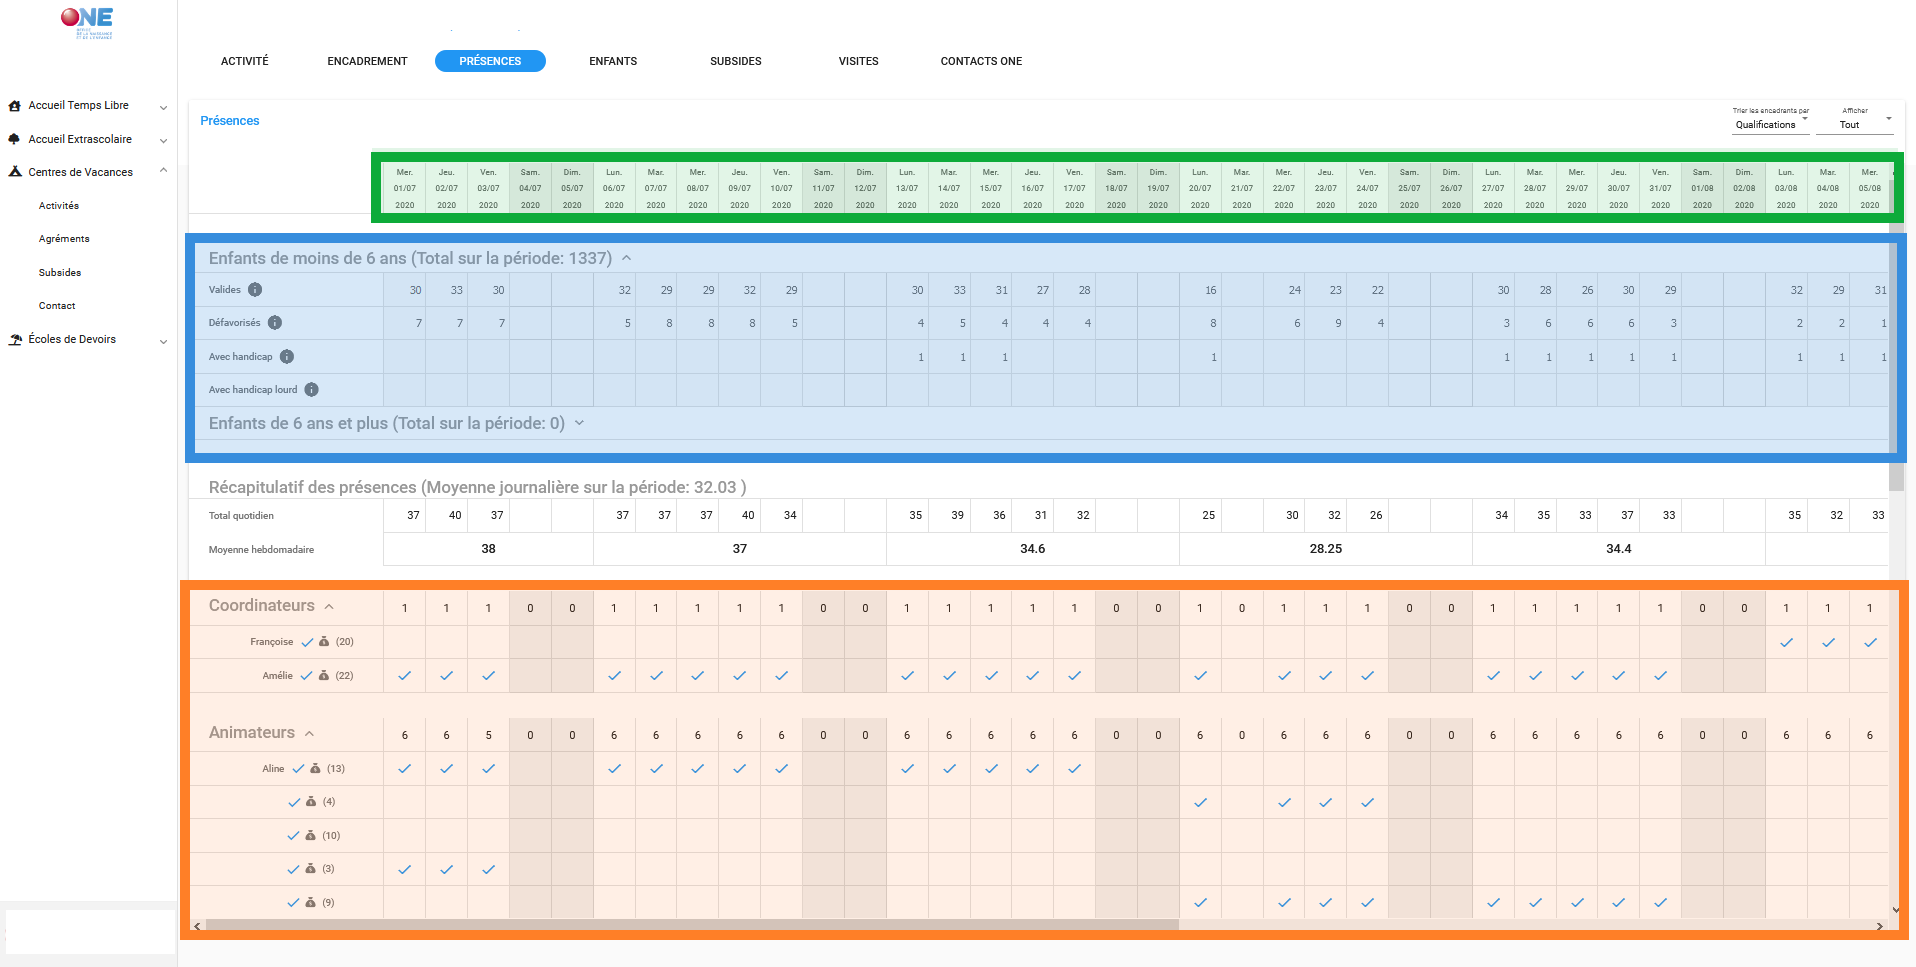
\includegraphics[width=18cm]{Images/cdv/cdv-ds-presences.png}}

\begin{info}
La grille de présence rependra les dates de votre déclaration d'activité (onglet \ovalbox{activité}). S'il manque des jours, contactez votre gestionnaire pour qu'il puisse mettre à jour les dates de votre centre de vacances. 
\end{info}

\subsubsection{Présences des enfants}
\underline{Il y a deux groupes d'âge pour les enfants:}

\begin{itemize}
    \item \textbf{Les moins de six ans}: reprend les enfants de 30 mois à 5 ans.
    \item \textbf{Les plus de six ans}: reprend les enfants de 6 à 15 ans. Les enfants en situation de handicap peuvent être repris jusqu'à l'âge de 21 ans.
\end{itemize}

\underline{Chaque groupe d'âge est ventilé selon les catégories suivantes:}
\begin{itemize}
    \item \textbf{valides}: les enfants qui ne rentrent dans aucune des catégories ci-dessous. 
    \item \textbf{défavorisés}: est considéré comme enfant issu de milieu socio-économique défavorisé, l'enfant âgé de 30 mois à 15 ans appartenant à un milieu familial précarisé où au moins un des parents ayant effectivement l'enfant à sa charge bénéficie d'un revenu de remplacement ou est exclu des mécanismes de protection sociale.
    \item \textbf{avec handicap}: par enfant en situation de handicap léger, il faut entendre le participant au centre de vacances âgé de 30 mois à 21 ans qui ne nécessite pas d'aide ou une aide partielle pour se laver, s'habiller, se déplacer, aller aux toilettes, se nourrir, communiquer ou avoir conscience des dangers.
    \item \textbf{avec handicap lourd} \textit{(ne concerne que les centres spécialisés)}: par enfant en situation de handicap lourd, il faut entendre le participant qui nécessite davantage d'aide ou une aide complète dans les activités du centre et de la vie quotidienne.
\end{itemize}

\begin{tcolorbox}[title=Comment encoder les présences des enfants ?]
Indiquez le nombre total d'enfants par tranche d'âge et par catégorie pour chaque journée. Un enfant ne doit être repris que dans une seule catégorie. Les week-end apparaissent en grisé, mais vous pouvez encoder des présences (séjour). L'enregistrement se fait automatiquement.

\end{tcolorbox}

\subsubsection{Présences des encadrants}
Le personnel repris dans l'onglet \ovalbox{Encadrement} est repris par fonction (coordinateur ou animateur). Pour ajouter un membre du personnel, référez-vous au point \hyperref[encadrementcdv]{"DS (1/4) ‐ L’onglet Encadrement"} du guide.

\begin{tcolorbox}[title=Comment encoder les présences des encadrants ?]
Cliquez sur la case du jour pour confirmer que la personne était bien présente. Un petit {\color{bleu}V} apparaîtra. Si une personne a été encodée pour deux fonctions (animateur - coordinateur), elle apparaîtra une première fois dans la section "coordinateur" et une deuxième fois dans "animateur"; par contre, elle ne peut endosser qu'un rôle pour un même jour. 
\end{tcolorbox}

\subsection{DS (3/4) - L'onglet Enfants}
Il y a deux parties dans cet onglet: la \textcolor{bleu}{liste des enfants à charger} et le \textcolor{ocre}{récapitulatif du nombre d'enfants} pour lesquels le subside est demandé. 

\begin{figure}[h]
    \centering
    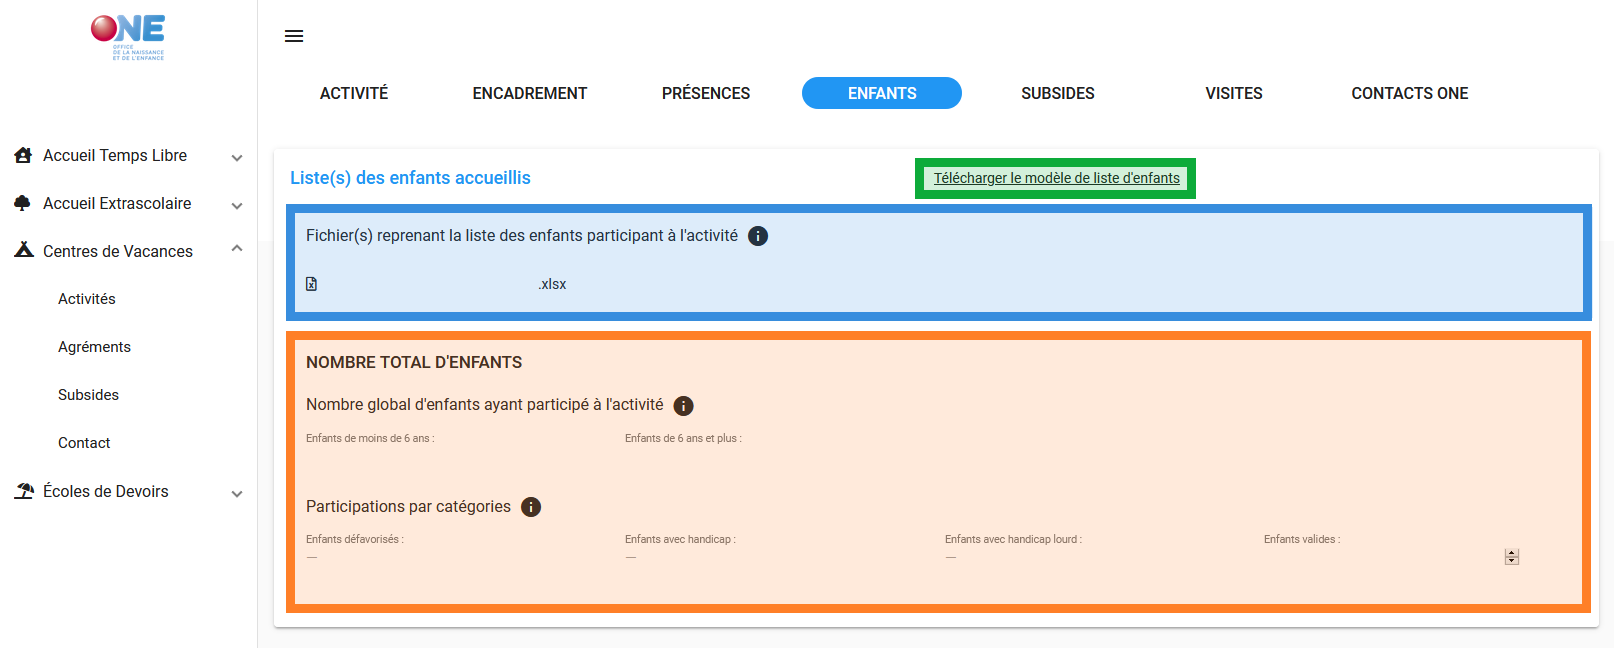
\includegraphics[width=15cm]{Images/cdv/cdv-ds-enfants.png}
    \caption{Onglet Enfants: chargez le fichier de liste d'enfants et les nombre total d'enfants. Un modèle Excel est disponible en téléchargement. Vous pouvez utiliser ce modèle ou utiliser votre propre format de fichier à condition de reprendre tous les éléments du modèle de références et respecter l'ordre et la forme du contenu.}
    \label{fig:cdv_enfants}
\end{figure}


\subsubsection{Liste des enfants accueillis}
La première partie consiste à charger la liste des enfants. 


\subsubsection{Récapitulatif du nombre d'enfants}
Pour modifier cette seconde partie, cliquez sur le crayon de modification. Indiquez le nombre d'enfants pour chaque tranche d'âge et pour chaque catégorie (cf. définition dans le point \ref{cdv_présence} du guide). Pour rappel, un enfant ne doit être repris que dans une seule catégorie.

N'oubliez pas de cliquer sur \ovalbox{Enregistrer} pour valider vos modifications. 


\subsection{DS (4/4) - L'onglet Subsides}
Lorsque les onglets \ovalbox{Encadrement}, \ovalbox{Présences}, \ovalbox{Enfants} ont été complètement remplis, vous pouvez procéder à l'envoi de la demande de subsides. Cochez les cases "attestation sur l'honneur" et cliquez ensuite sur \ovalbox{Envoyer ma demande de subsides} (figure \ref{fig:cdv_subsides}). 

\begin{figure}[h]
    \centering
    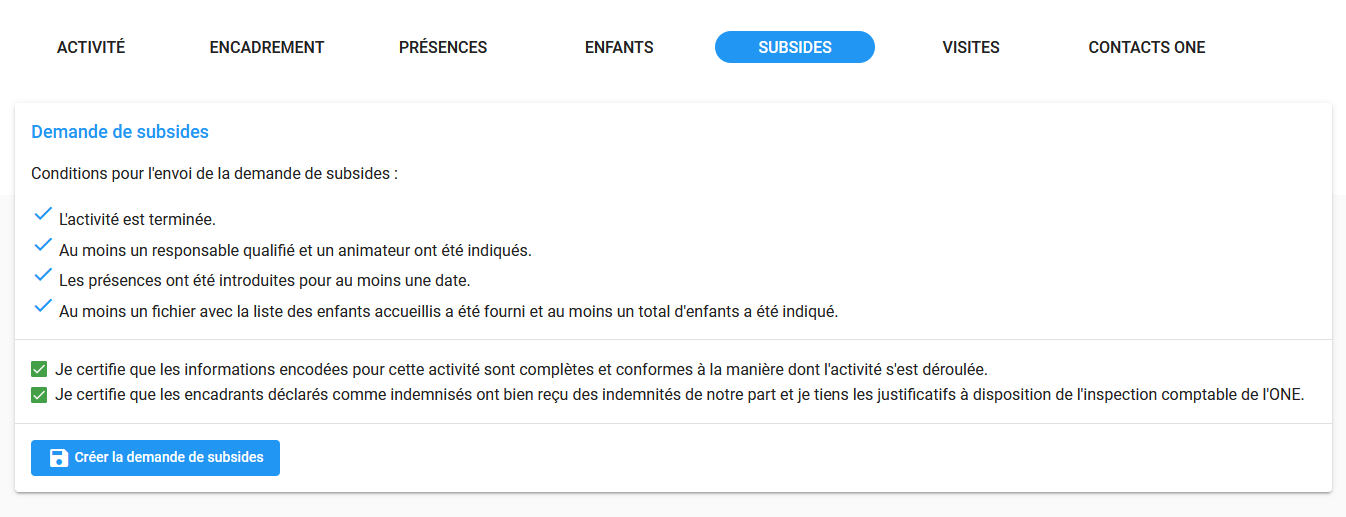
\includegraphics[width=12.5cm]{Images/cdv/cdv-ds-subsides.png}
    \caption{Onglet Subsides: le bouton 'Envoyer' la demande de subsides est disponible si les conditions décrites sont remplies.}
    \label{fig:cdv_subsides}
\end{figure}


Une fois votre demande de subsides envoyée, l'onglet \ovalbox{Subsides} affichera la date d'envoi. Si vous souhaitez rectifier votre demande de subsides (encadrement, présences ou enfants), contactez votre gestionnaire de dossiers afin qu'il puisse rouvrir l'édition de votre demande de subsides. 
\begin{information}
Il est toujours possible d'ajouter des pièces justificatives pour la qualification de vos encadrants, et ce même si la demande de subsides a déjà été envoyée.
\end{information}